En este apartado se abordará el diseño físico de datos del sistema, que se encarga de definir cómo se almacenarán los datos en la base de datos.

\subsubsection{Descripción del SGBD utilizado}
Para el almacenamiento de los datos se ha utilizado el sistema de gestión de bases de datos (SGBD) MongoDB, que es una base de datos NoSQL orientada a documentos.
Concretamente se ha utilizado su versión en la nube, MongoDB Atlas.

MongoDB es una base de datos NoSQL que almacena los datos en documentos BSON (Binary JSON), que son una representación binaria de JSON.
Estos documentos se almacenan en colecciones, que son agrupaciones de documentos.

MongoDB es una base de datos muy flexible, ya que no requiere que los documentos de una misma colección tengan la misma estructura.
Aún así, en este proyecto se ha definido una estructura fija para los documentos de cada colección, para facilitar la gestión de los datos.

La integración de MongoDB Atlas en el proyecto se ha realizado mediante la librería Mongoose.

\subsubsection{Documentos definidos}
A continuación se detallan los documentos definidos para cada colección de la base de datos junto con una breve descripción de cada uno.

\begin{itemize}

    \item \textbf{Auction (Subasta)}: Representa una subasta donde se subasta una carta de usuario (UserCard).

    \item \textbf{UserCard (Carta de Usuario)}: Representa una carta de Pokémon que pertenece a un usuario.

    \item \textbf{User (Usuario)}: Representa un usuario del sistema.

    \item \textbf{Bid (Puja)}: Representa una puja realizada por un usuario en una subasta.

    \item \textbf{Card (Carta)}: Representa una carta de Pokémon con detalles específicos sobre el Pokémon, la carta y sus transacciones.

    \item \textbf{CardPack (Sobre de Cartas)}: Representa un sobre de cartas de Pokémon que contiene varias cartas.

    \item \textbf{Deck (Mazo de cartas)}: Representa un mazo de cartas que agrupa varias cartas de Pokémon.

    \item \textbf{Notification (Notificación)}: Representa una notificación enviada a un usuario.

    \item \textbf{Transaction (Transacción)}: Representa una transacción que involucra la compra o venta de una carta de usuario (UserCard).

\end{itemize}

También se han definido enumeraciones para los campos que requieren un valor de una lista predefinida, como el estado de una subasta o el tipo de una carta.
Estos campos se almacenan como cadenas de texto en la base de datos, pero se han definido enumeraciones en el código para facilitar su uso. Estos son:

\begin{itemize}
    \item \textbf{AuctionStatus (Estado de Subasta)}: Enumera los posibles estados de una subasta.

    \item \textbf{BidStatus (Estado de Puja)}: Enumera los posibles estados de una puja.

    \item \textbf{CardRarity (Rareza de Carta)}: Enumera los diferentes niveles de rareza de una carta de Pokémon.

    \item \textbf{PokemonType (Tipo de Pokémon)}: Enumera los diferentes tipos de Pokémon.

    \item \textbf{PokemonGym (Gimnasio Pokémon)}: Enumera los diferentes gimnasios Pokémon donde pueden encontrarse los Pokémon.

    \item \textbf{NotificationType (Tipo de Notificación)}: Enumera los diferentes tipos de notificaciones.

    \item \textbf{NotificationImportance (Importancia de la Notificación)}: Enumera los diferentes niveles de importancia de una notificación.

    \item \textbf{TransactionConcept (Concepto de Transacción)}: Enumera los diferentes conceptos para las transacciones realizadas.
\end{itemize}


\subsubsection{Modelo de datos}
A continuación se muestra el modelo de datos de la base de datos, que representa las colecciones y los campos de cada documento.

\begin{figure}[H]
    \centering
    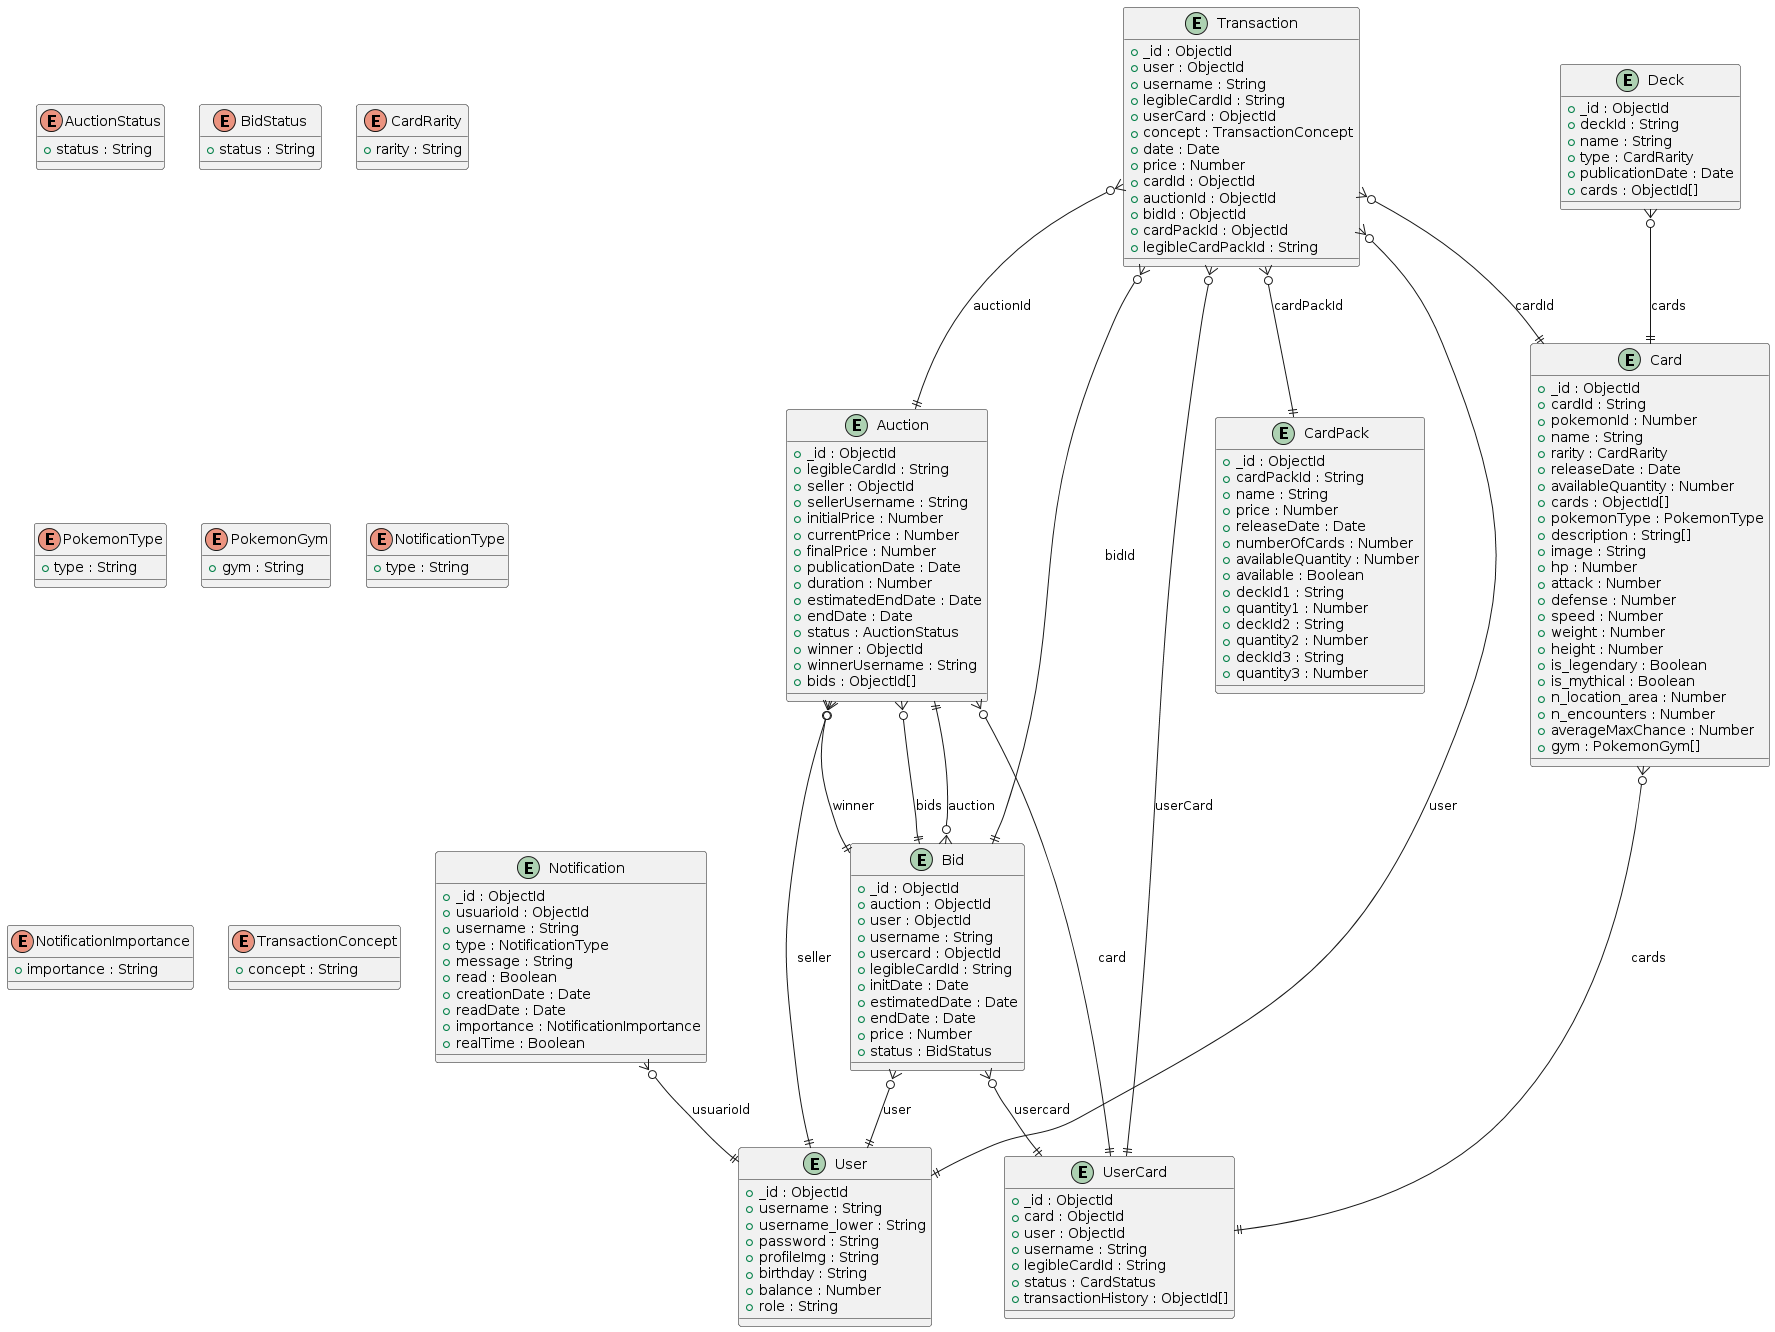
\includegraphics[width=1\textwidth]{figures/6-Analisis/6_9_mongodb_model.png}
    \caption{Modelo de datos de la base de datos MongoDB}
    \label{fig:mongodb_model}
\end{figure}
